\documentclass[12pt]{article}

\usepackage[english, russian]{babel}
\usepackage[left=2.8cm,right=2.8cm, top=2.8cm,bottom=2.8cm,bindingoffset=0cm]{geometry}
\usepackage{amsmath,amsfonts,amssymb,amsthm,mathtools}
\usepackage[pdftex]{graphicx}
\usepackage{hyperref}
\usepackage{xcolor}
\usepackage{ulem}
\everymath{\displaystyle}


\begin{document}


\begin{center}
Расшариваю Акос. \\
\textcolor{blue}{\href{https://t.me/oleander_twig}{oleander\_twig}}
\end{center}

\tableofcontents
\section{Введение.}

\subsection{Архитектура фон Неймана}
Современные компьютеры устроены сейчас примерно так: \\
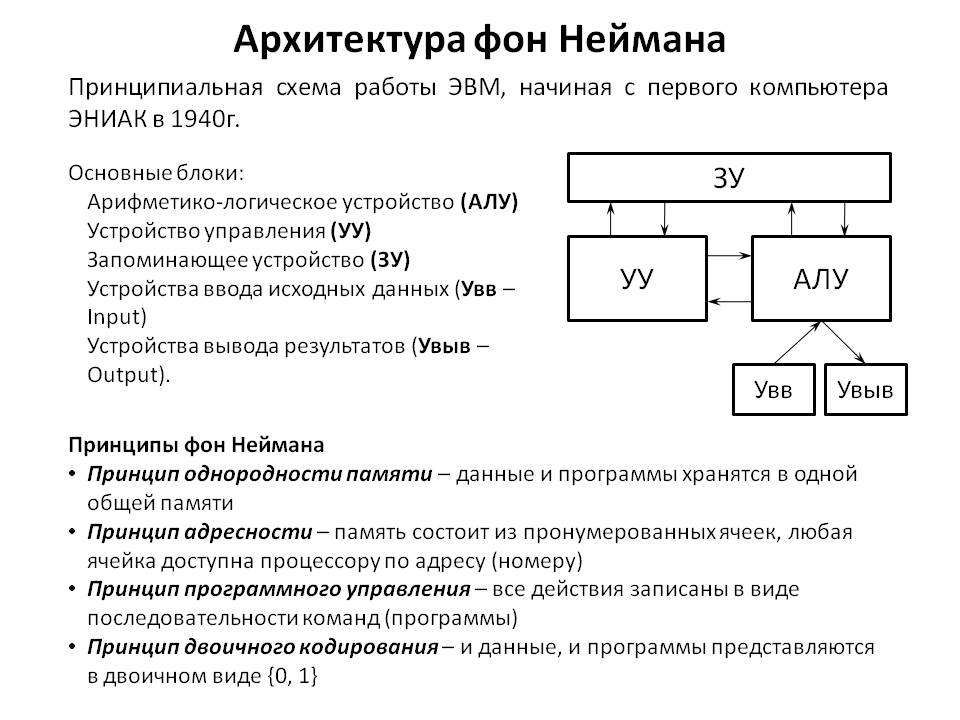
\includegraphics[scale=0.5]{./004.png} \\

\subsection{POSIX-ориентированные операционные системы.}
Все ОС делятся на Windows и POSIX-ориентированные ОС. \\
POSIX (англ. Portable Operating System Interface — переносимый интерфейс операционных систем) — набор стандартов, описывающих интерфейсы между операционной системой и прикладной программой (системный API), библиотеку языка C и набор приложений и их интерфейсов. Стандарт создан для обеспечения совместимости различных UNIX-подобных операционных систем и переносимости прикладных программ на уровне исходного кода, но может быть использован и для не-Unix систем. \\
\\
\sl Основная задача - содействовать облегчению переноса кода прикладных программ на иные платформы. \\

\subsection{ОС семейства UNIX}
\rm Unix  — семейство переносимых, многозадачных и многопользовательских операционных систем. \\
\\
{ \sl Операционные системы семейства Unix характеризуются модульным дизайном, в котором каждая задача выполняется отдельной утилитой, взаимодействие осуществляется через единую файловую систему, а для работы с утилитами используется командная оболочка.} \\
\\
В ходе разработки Unix-систем был создан язык Си. \\
В настоящее время Unix-системы распространены в основном среди серверов, а также как встроенные системы для различного оборудования, включая смартфоны. Также Unix-системы доминируют на суперкомпьютерах, в частности, на $ 100\% $ суперкомпьютеров из рейтинга TOP500 установлена ОС Linux. \\
Среди ОС для рабочих станций и домашнего применения Unix и Unix-подобные ОС занимают после Microsoft Windows второе (macOS), третье (GNU/Linux) и многие последующие места по популярности. \\

\subsection{API операционных систем}

\section{Двоичная система счисления}
На самых низких уровнях ваш компьютер оперирует двоичным электрическим сигналом, который имеет только два состояния: есть ток или нет тока. Чтобы «понять» сложные данные, ваш компьютер должен закодировать их в двоичном формате – 1 и 0, соответствующим состояниям включения и выключения. 

\subsection{Беззнаковые числа}
Почти всегда, когда мы говорим "байт" мы НЕ подразумеваем 8 бит. \\
{\bf Байт} - минимально адресуемая единица памяти. По стандартам си/си++ в роли байта выступает {\bf char}. 

\begin{verbatim}
sizeof (char) == 1;
\end{verbatim}

Все прочие размеры объектов си измеряются в единицах типа char. \\ Количество бит в char определяется константой {\bf \textcolor{magenta}{CHAR\_BIT}}. 

\begin{verbatim}
sizeof(sighned T) == sizeof(unsighned T) ==sizeof(T);
\end{verbatim}

{\sl На крайняк всегда можно сделать printf константы.} \\
\\
Беззнаковые числа имеют диапозон представимых значений $[0; 2^{N - 1}], \; N$ - число быит. 

\begin{verbatim}
0 - 1U = UINT_MAX;
\end{verbatim}
Приписывая суффикс $"u"$, мы даём программе понять, что операция должна восприниматься как беззнаковая. 

\subsection{Битовые маски.}
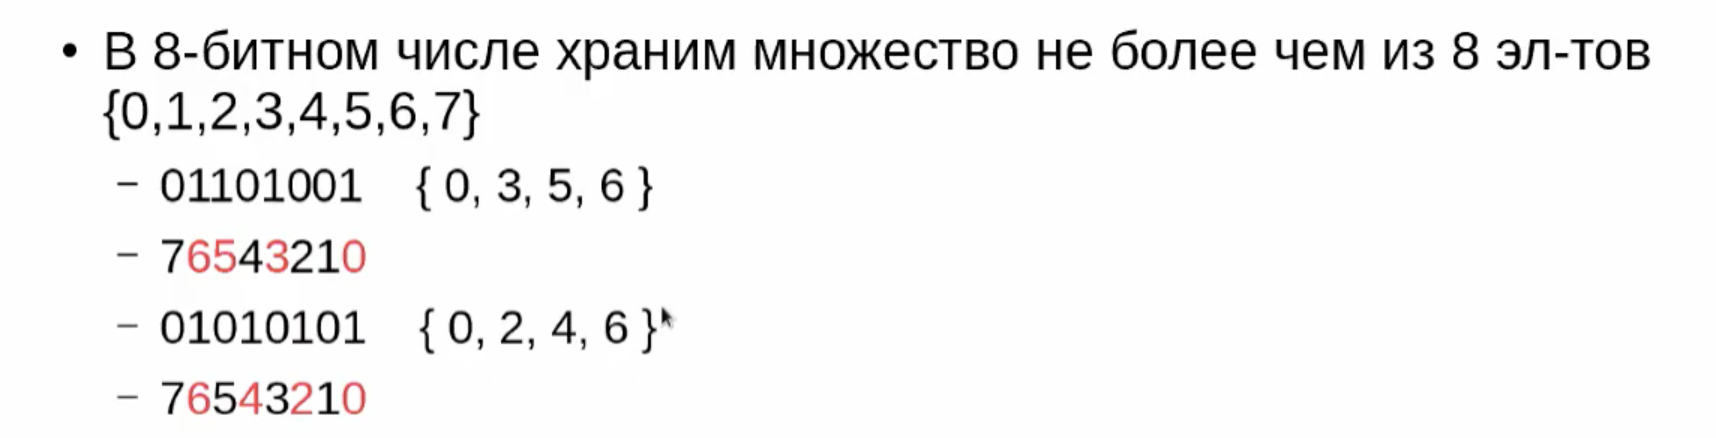
\includegraphics[scale=0.5]{./masks.png} \\

\subsection{Сдвиги в беззнаковых числах}
Сдвиг {\bf влево} для числа x = 01101100 на n = 3: 
$$ 01101100 << 3 := \xout{011}01100 \textcolor{blue}{000} $$
По сути, сдвиг влево эквивалентен умножению на $2^{n}$. \\
\\
Сдвиг {\bf вправо} для числа x = 01101100 на n = 4:
$$ 01101100 >> 4 := \textcolor{blue}{0000}0110\xout{1100} $$
По сути, сдвиг вправо эквивалентен целой части от деления на $2^{n}.$

\subsection{Знаковые числа}
Стандарты Си/Си++ допускают три типа представления знаковых чисел: \\
1) Прямой код; \\
2) Обратный код (число с противоположным знаком - обитовое отрицание); \\
3) Дополнительный код. \\
Самым распространённым является дополнительный код. Мы тоже будем его использовать. \\
\\
{\bf Дополнительный код:} \\
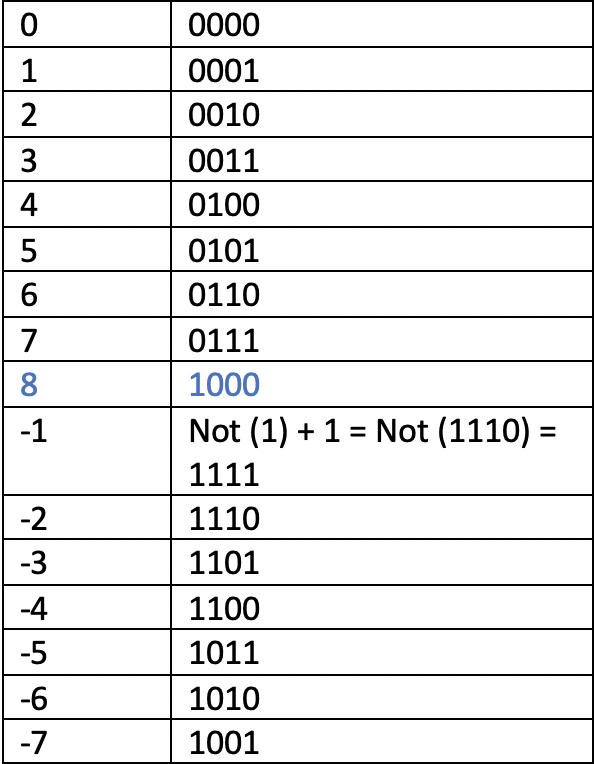
\includegraphics[scale=0.5]{./30.11.png} \\

\subsection{Расположение байтов в памяти}
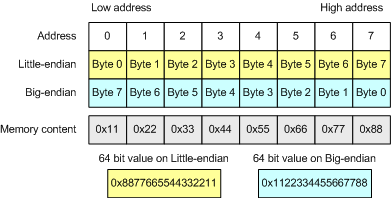
\includegraphics[scale=1]{./4.png} \\

\subsection{Преобразование беззнаковых чисел в знаковые и наоборот}
Знаковый $\longrightarrow$ беззнаковый. 

\begin{verbatim}
int main() {
    int a = -6;
    unsigned int b;
    b = ~(a) + 1;
    printf("%u\n", b);
}
\end{verbatim}

Беззнаковый $\longrightarrow$ знаковый. 

\begin{verbatim}
int main() {
    int a;
    unsigned int b = 9;
    a = ~b + 1;
    printf("%d\n", a);
}
\end{verbatim}

\section{Дробные числа с фиксированной точкой.}
\subsection{Представление чисел}
Полезная презентация: 
\textcolor{blue}{\href{https://www.cs.cmu.edu/afs/cs/academic/class/15213-f15/www/lectures/04-float.pdf}{cs.cmu.edu}} \\
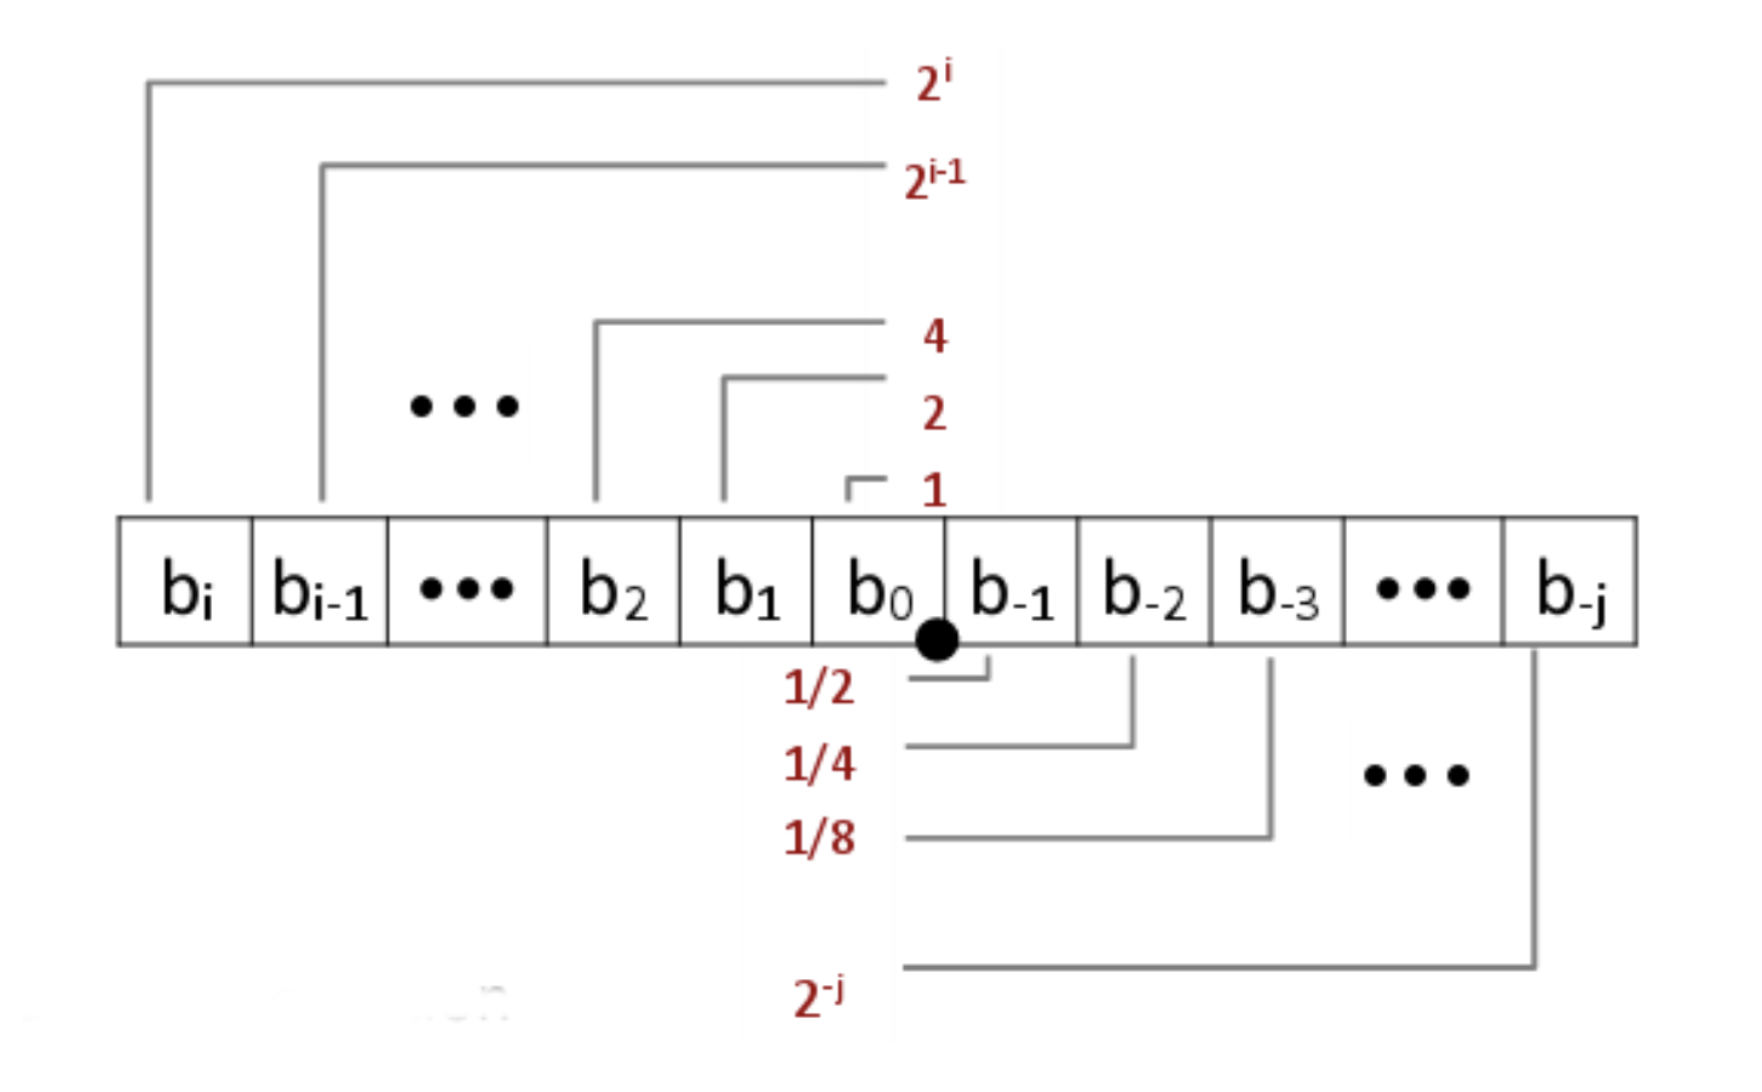
\includegraphics[scale=0.5]{./floating_point.png} \\

То есть наше число представимо в десятичном виде следующим образом: $\sum_{k = -j}^{i} b_{k} \cdot 2^{k}$

Например, \\
Число $5\dfrac{3}{4} = 5. 75$ представимо в двоичной системе как $101.11_{2} = 1 \cdot 2^{2} + 0 \cdot 2^{1} + 1 \cdot 2^{0} + 1 \cdot 2^{-1} + 1 \cdot 2^{-2} = 5 + \dfrac{1}{2} + \dfrac{1}{4}$.

Понятно, что не всегда преобразование из десятичной записи может быть выполнено точно. Например, $ 10 = 2\cdot 5 $ 
$$ \dfrac{1}{5} = 0.2 \approx 00000011_{2} = 0.1875$$ 
то есть $\dfrac{1}{5}$ - это бесконечная периодическая двоичная дробь: $0.001100110011[0011]..$. 

Еще одна такая дробь это $0.1_{10} = 0.0001100110011[0011]..$ . Посмотрим повнимательнее: $00000010_{2} = 0.125$, ошибка составила $|0.1 - 0.125| = 0.025.$ \\
$00000001_{2}= 0.0625$, ошибка: 0.0375 - хуже, чем 0.025. 

Обратим внимание на то, что 0.0625 - вес младшего разряда (ULP). \textbf{Ошибка преобразования не должна превышать половины веса младшего разряда (ULP/2 = 0.03125)}.

\subsection{Операции над числами}

\textbf{Сложение} и \textbf{вычитание} производятся как с целыми числами. \\
\textbf{Умножение} в общем случае работает так же как и с целыми числами. Только при умножении n-битных чисел мы получим 2n-битное. Его потом следует округлить до n-битного. Например, \\
$$ 0010.0110 \cdot 0100.0010 = 1001.11001100\approx 1001.1101 $$
Точный результат: 9.796875, а округлённый: 9.825. Убедимся, что ошибка (0.015625) не превысила $\text{ULP}/2 = 2^{-4}/2 = 0.125$.

\subsubsection*{Деление}
$$0100.0010_{2} \div 0010.0110_{2}=$$
1) Убираем точки в обоих числах; \\
1) Дополняем первое число справа 8 нулями, получаем 16-битное число $0100001000000000_{2} = 16896$; \\
2) Делим как целое: $16896 \div 38(00100110_{2}) = 444 = 110111100_{2}$; \\
3) Ставим точку на своё место $1.10111100_{2} = 1.734375$ и округляем $1.1100_{2} = 1.75$. 

Убедимся, что ошибка все еще не превышает  $\text{ULP}/2$. Итак, точные вычисления: $4.125 \div 2.375 = 1.73684..$; Ошибка: 0.013157..; $ \text{ULP}/2 = 0.125$. Ура!

\subsection{Округление}
Стандарт IEEE754 предусматривает четыре способа округления чисел: \\
1) Округление, стремящееся к ближайшему целому; \\
2) Округление, стремящееся к нулю; \\
3) Округление, стремящееся к $+\infty$; \\
4) Округление, стремящееся к $-\infty$. \\
По умолчанию округление происходит по первому способу. Часто в различных устройствах используют второй способ - округление к нулю. При округлении к нулю нужно просто отбросить не значащие разряды числа, поэтому этот способ самый легкий в аппаратной реализации. \\
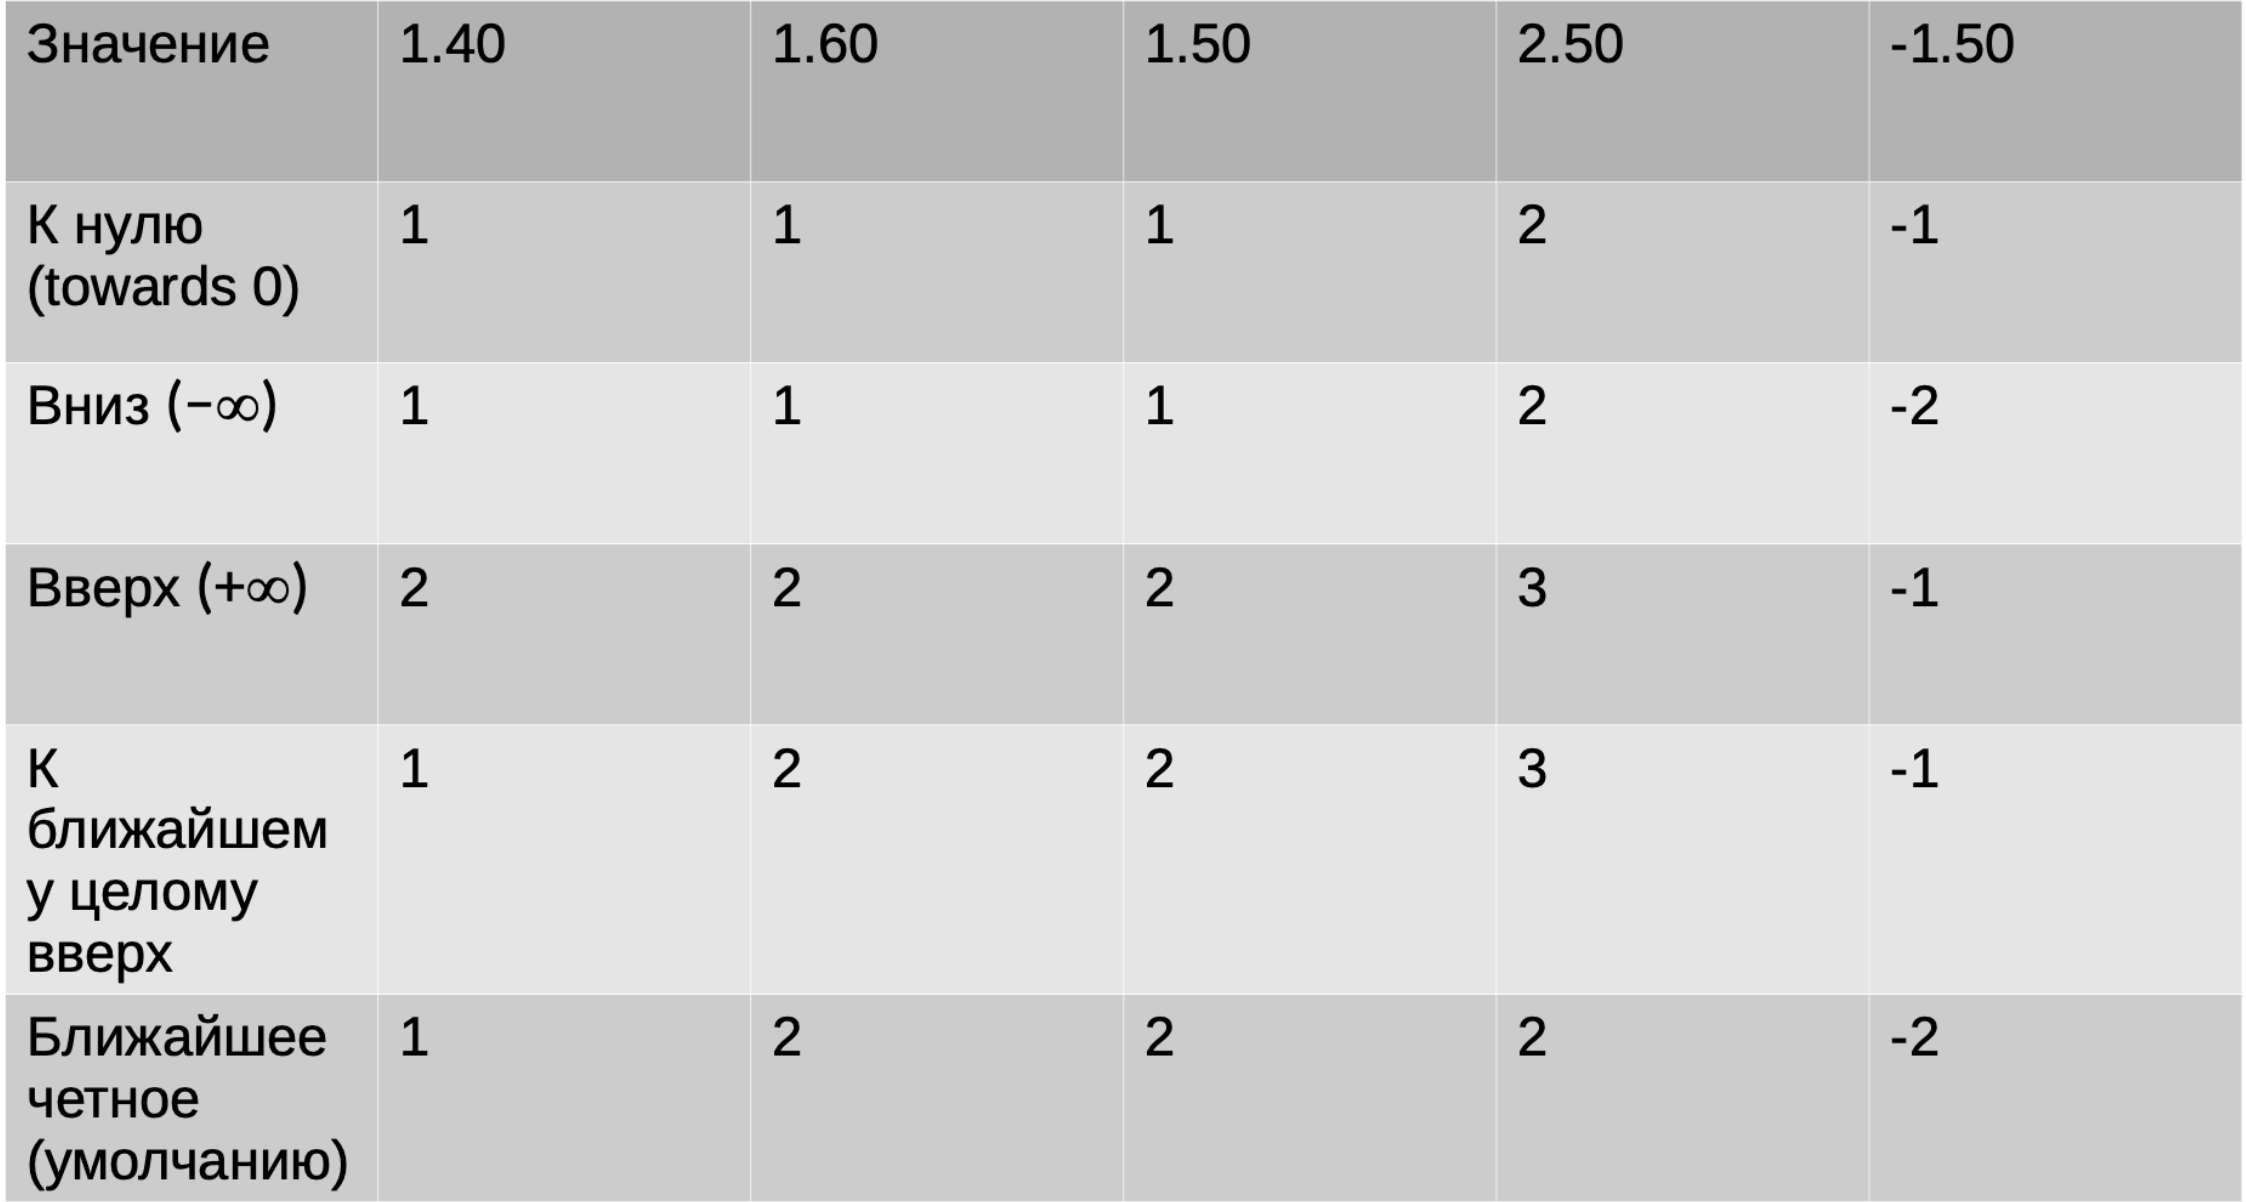
\includegraphics[scale=0.4]{./round.png} 

\section{Дробные числа с плавающей точкой.}
Еще одна полезная презентация: \textcolor{blue}{\href{https://www.softelectro.ru/ieee754.html}{https://www.softelectro.ru/ieee754.html}}

\subsection{Представление чисел}

\subsubsection*{Стандарт IEEE 754}
Данный стандарт разработан ассоциацией IEEE (Institute of Electrical and Electronics Engineers) и используется для представления действительных чисел (чисел с плавающей точкой) в двоичном коде. \\
\\
\textbf{Числовая форма: $ (-1)^{s} M 2^{E}$}, где \\
s определяет знак числа; \\
M - мантисса, значение которой обычно лежит в диапозоне $[1.0; 2.0)$. 

\subsubsection*{Представление числа}
Тут s - кодирование знака, exp - кодирование E (порядка), frac - кодирование мантиссы. \\
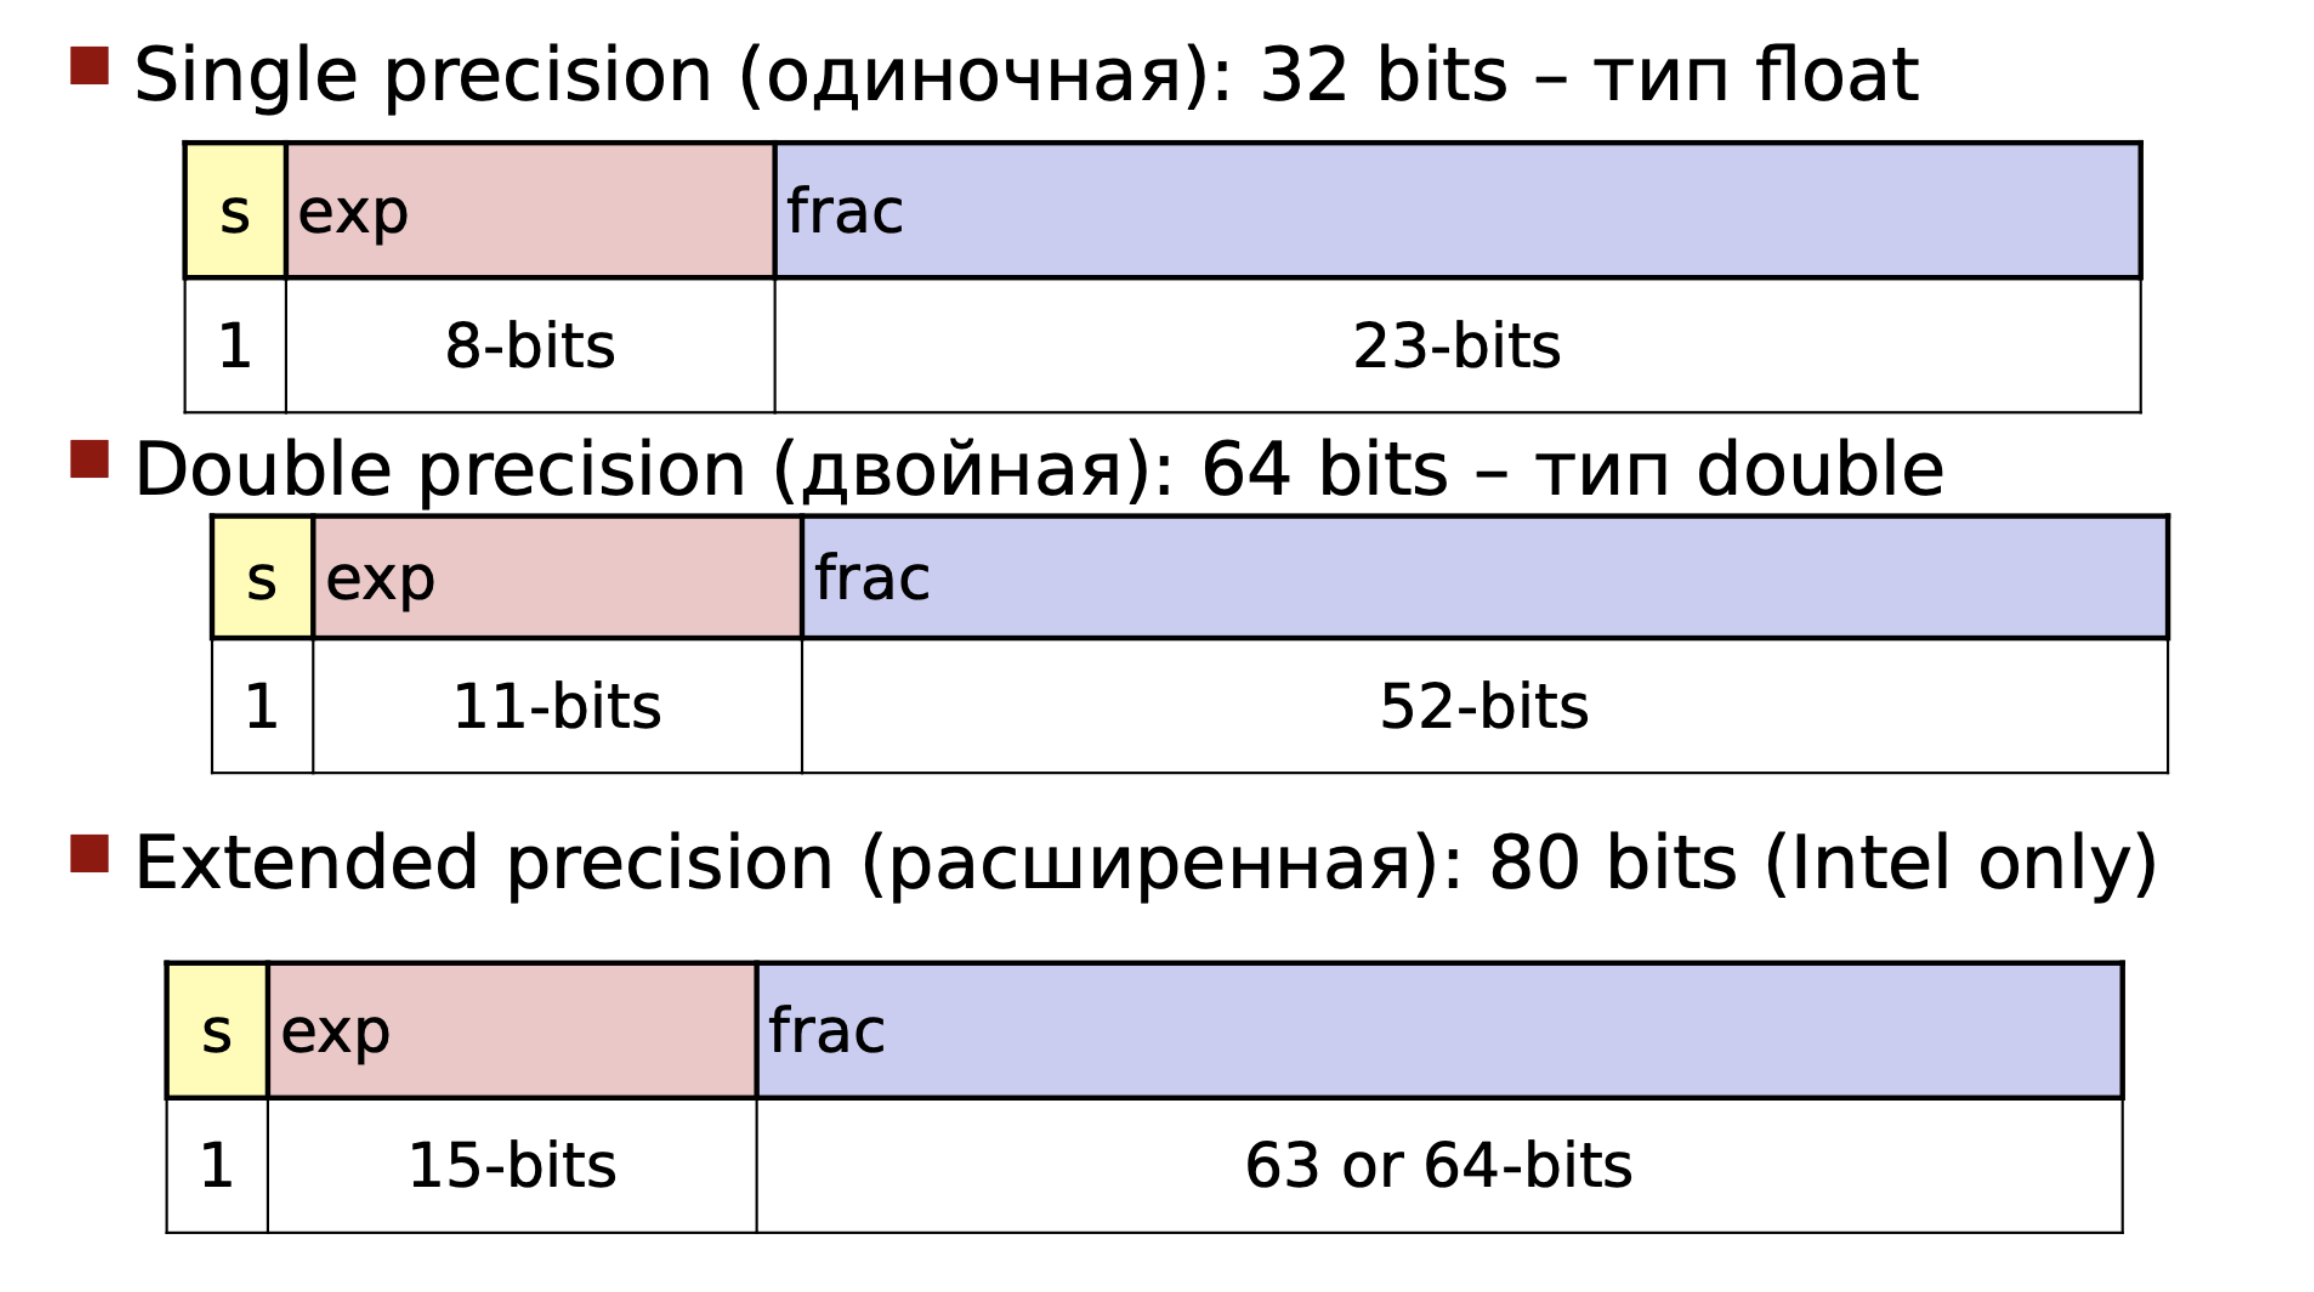
\includegraphics[scale=0.4]{./encoding.png} \\

Число считается \textbf{нормализованным} $\Leftrightarrow$ \\
1) $\text{exp} \neq 0 ... 0 \; \text{and exp} \neq 1 ... 1$; \\
2) порядок кодируется со смещением : E = exp - bias, где exp - беззнаковое значение, bias $= 2^{k - 1}, k \; - $ число бит порядка; \\
3) мантисса кодируется со "скрытой" ведущей $1:M = 1.xxxx_{2}$, где xxxx - биты мантиссы (frac); min frac = 0 ... 0, max frac = 1 ... 1.  \\

Число считается \textbf{денормализованным} $\Leftrightarrow$ \\
1) $\text{exp} \neq 0 ... 0$; \\
2) порядок кодируется со смещением : E = 1 - bias; \\
3) мантисса кодируется со "скрытой" ведущей $0:M = 1.xxxx_{2}$, где xxxx - биты мантиссы (frac). 

\subsection{Операции с плавающей точкой}
\underline{Основная идея:} \\
$\bullet$ Сначала вычиляем точный результат; \\
$\bullet$ Потом помещаем требуемую точность. 

\subsubsection*{Умножение}
$$(-1)^{s1}M1 \; 2^{E1} \cdot (-1)^{s2}M2 \; 2^{E2} = $$
Точный результат: $(-1)^{(s1)^{s2}}\; (M1 \cdot M2) \; 2^{E1 + E2} $ \\
Корректируем: Если $M \geqslant 2$, то сдвигаем M вправо, увеличиваем E. Если E вылезло из диапозона значений, значит случилось переполнение. Затем окргляем M так, чтобы добиться максимальной точности. 

\subsubsection*{Сложение}
 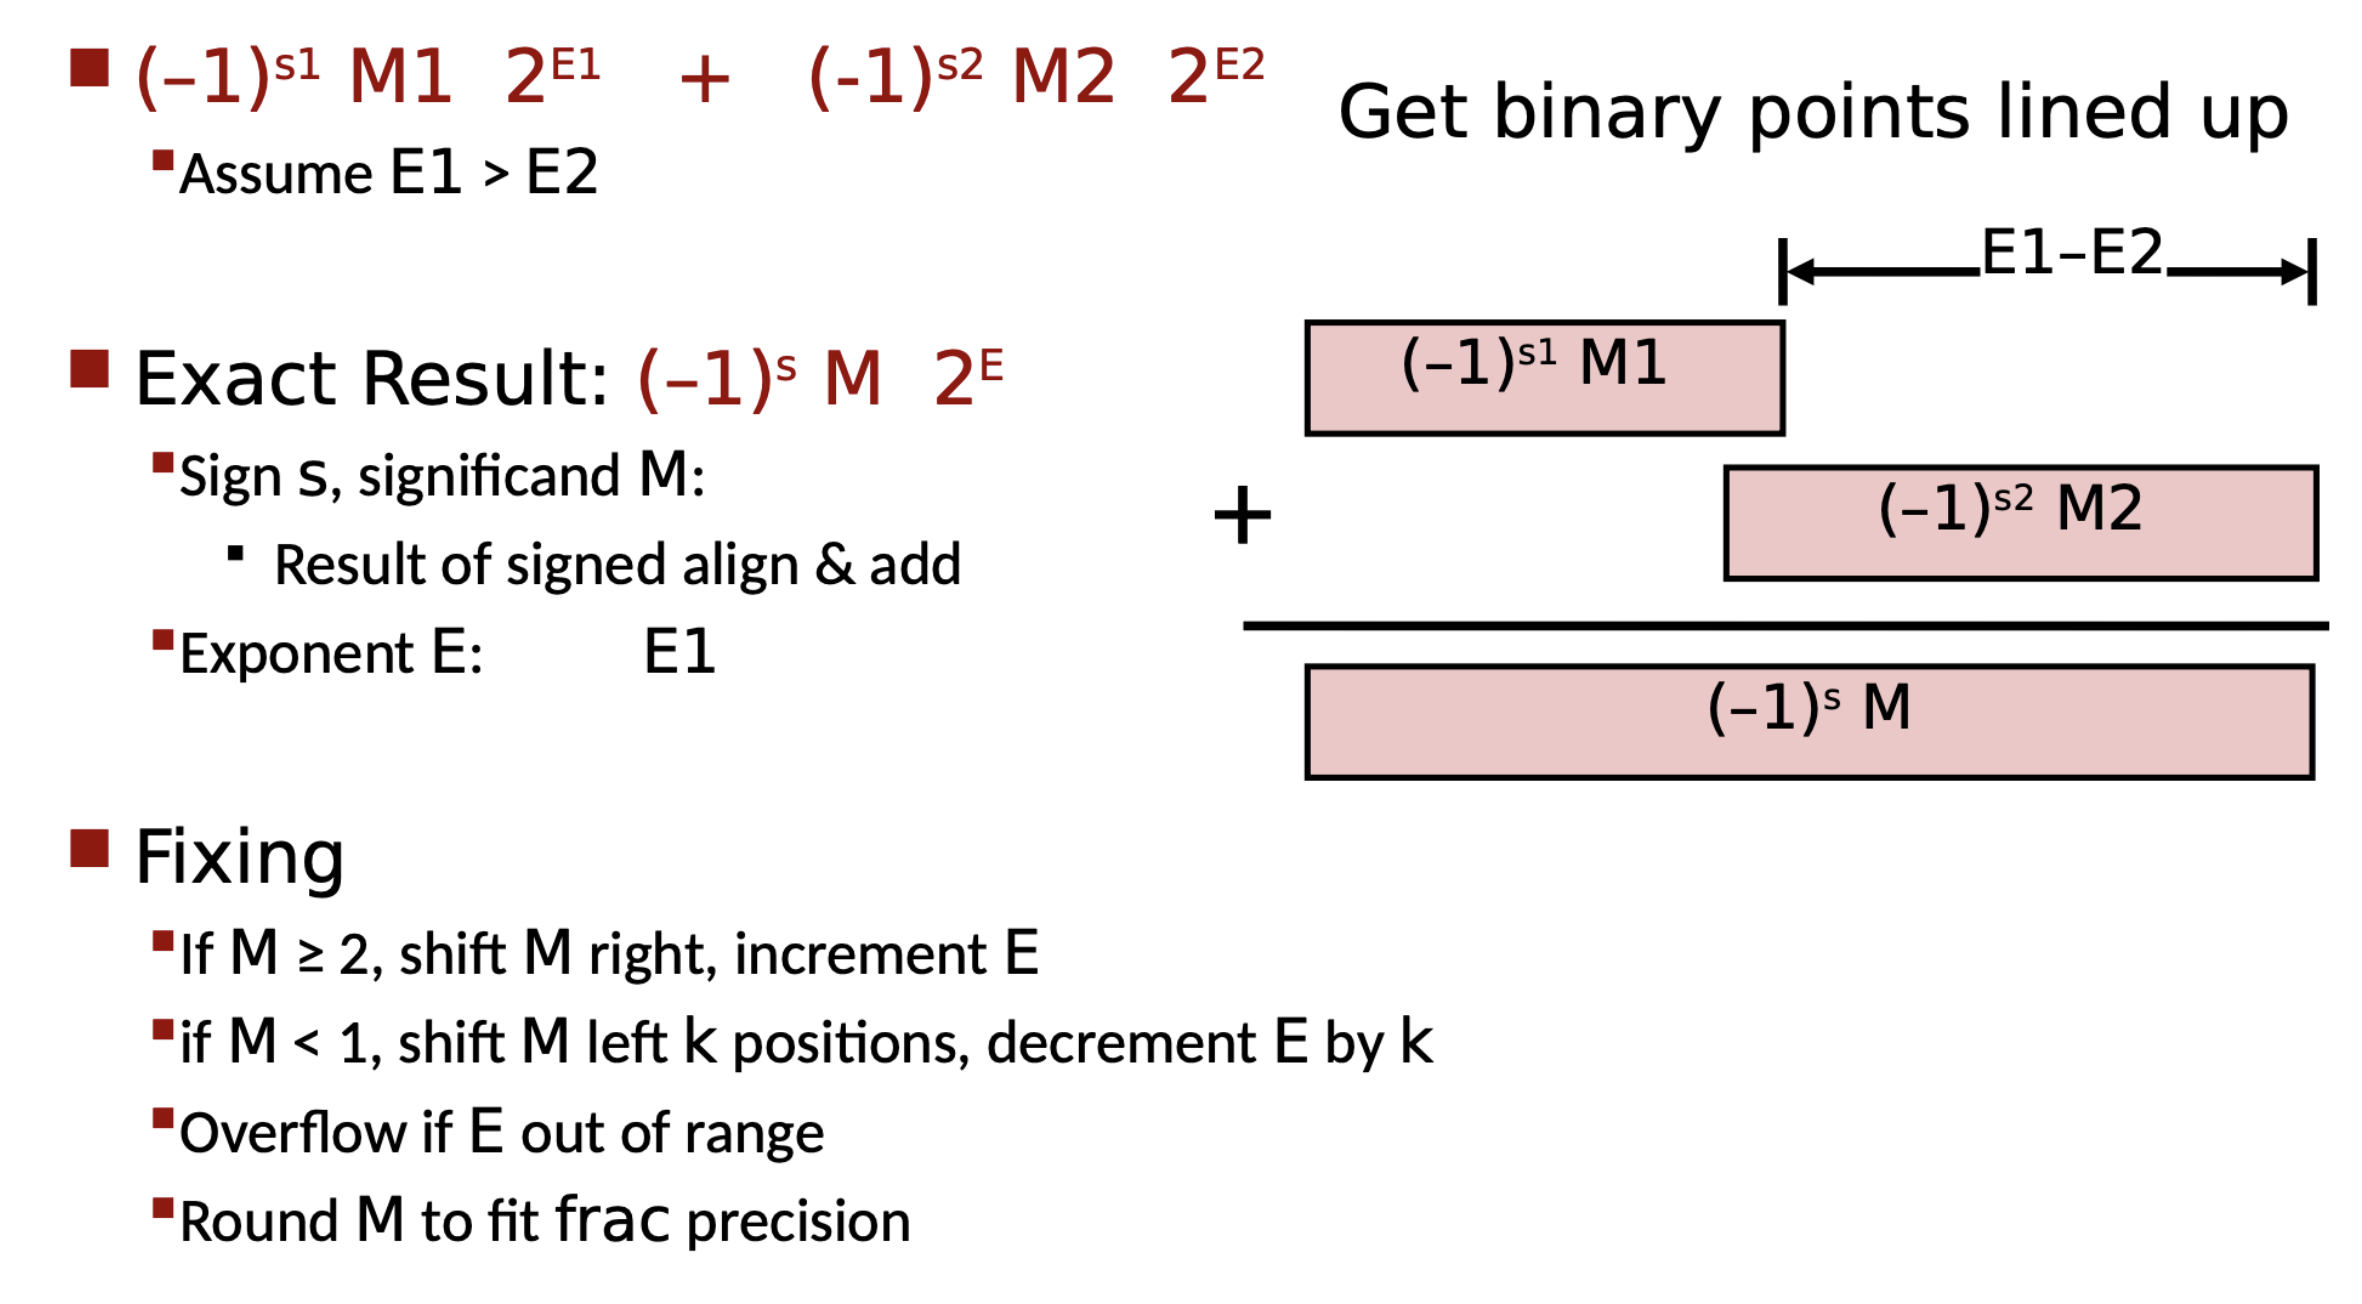
\includegraphics[scale=0.4]{./addition.png} \\
 Понятно, что знак одинаковый, иначе это вычетание. Итоговая матисса получается склеиванием двух изначальных, как показано на рисунке выше.

Чтобы минимизировать эффект от потери точности, последовательность вещественных чисел следует складывать следующим образом: \\
1) Положительные числа в порядке возрастания; \\
2) Отрицательные числа в порядке убывания; \\
3) Сложить два результата сложения, полученных выше чисел. 
 
 \subsection{Свойства операций}
  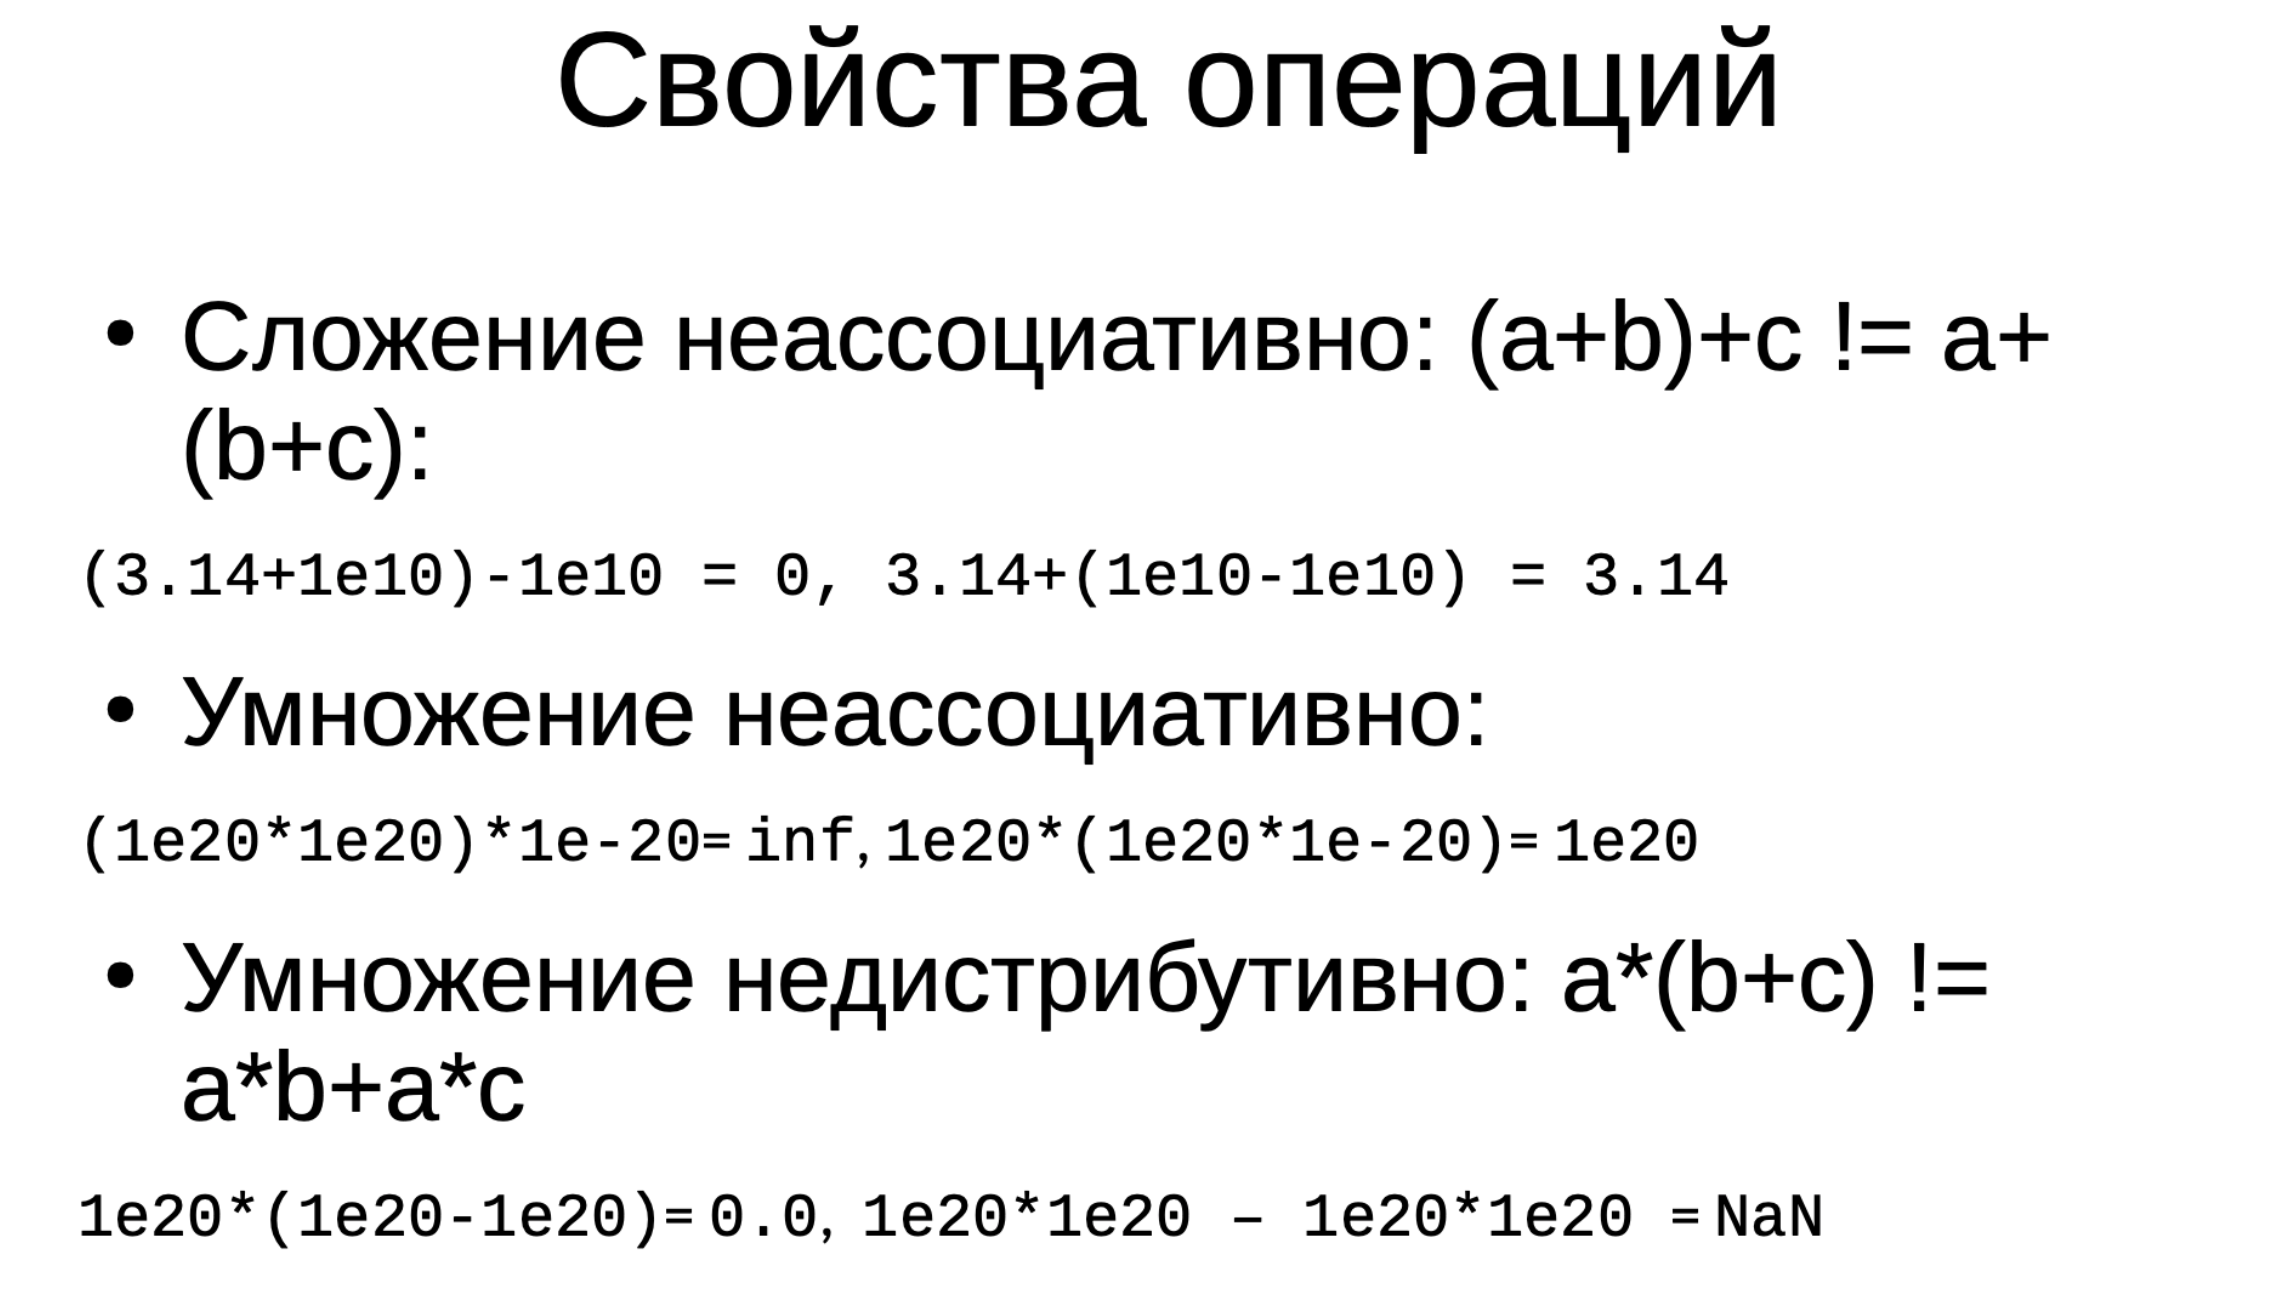
\includegraphics[scale=0.4]{./pic01.png} 
  
  \section{Литералы}
 Литерал  - запись в исходном коде компьютерной программы, представляющая собой фиксированное значение. Бывают строковые литералы ($'\setminus n'$ ), числовые (цифры), логические (TRUE), а бывают битовые (магические константы). \\
 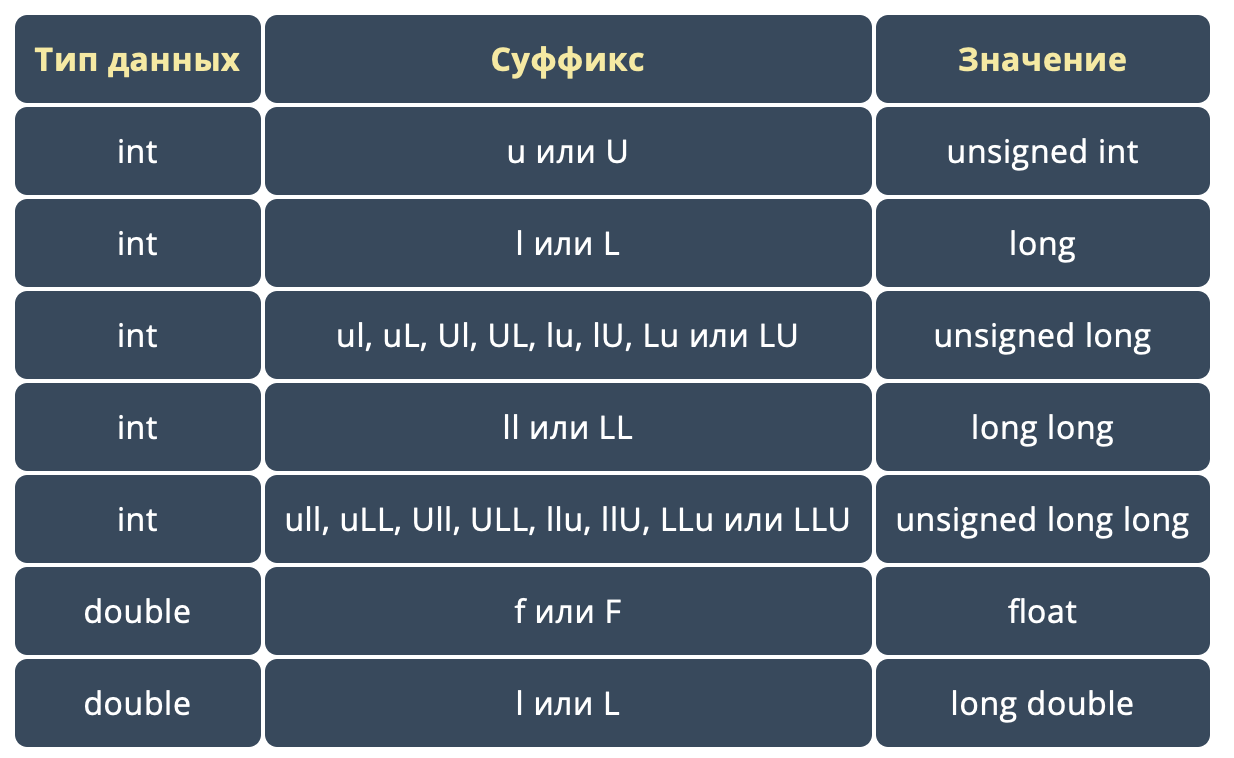
\includegraphics[scale=0.5]{./pic02.png} 
 
 Когда мы пишем $1ULL << n$ мы получаем единицу и n нулей после неё, само число помещается в $int64_t.$
 
 \section{Проект GNU}
 \textbf{Проект GNU} - свободное программное обеспечение (СПО). Проект был запущен Ричардом Столманом (Richard Stallman) в 1983. году.
 
 \textbf{4 свободы СПО:} \\
 1) Свобода выполнять программу как вам угодно  любых целях; \\
 2) Свобода изучать работу программы и модифицировать программу - предполагает доступ к исходному тексту; \\
 3) Свобода передавать копии ПО другим людям; \\
 4) Свобода передавать модифицированные копии ПО другим людям.
 \\ 
 \textbf{GNU Toolchain} - комплект утилитдля разработки рограммного обеспечения. В него входят: Gnu CompilerCollection (GCC), GNU Binutils (утилиты для работы с объектами  исполняемыми файлами в разных форматах), GNU Make (утилита для управления сборкой программ),GNU configure (утилита для конфигурирвания ПО). \\
 
 В GCC входят: \\
- \textbf{Драйвер компиляции} - небольшая программа, основная задача которой обработать аргументы командной строки и организовать процесс компиляции - вызов различных уже внутренних исполняемых программ (внутри gcc) в нужной последовательности для всех тех файлов, которые были перечислены в командой строке. Для каждого языка программирования - свой драйвер компиляции. Например, для С - это gcc; для С++ - это g++; Fortan - gfortran; Go - gccgo. \\
- собственные компиляторы языков (генерируют программу а языке асемблера). \\
- стандартный библиотеки языков С++ и Java. \\

\textbf{Шаги компиляции С и С++ программ:} \\
1) Препроцессирование (обработка всех include, раскрытие всех макросов (то есть define), условная компиляция, после препроцессирования файл имеет расширение .i) \\
2) Трансляция в ассемблер (после трансляции файл имеет расширение .s - это будет текстовый файл на языке ассемблера)\\
3) Ассемблирование (возвращает объектные файлы) \\
4) Компоновка (результат компоновки по умолчанию - файл a.out) и Link-Time optimizations . \\

\textbf{Объектный файл} - это бинарный файл, где инструкции ассемблера в текстовом виде заменены на инструкции ассемблера в бинарном виде (то есть применино байтовое кодирование к инструкциям), но это еще не полная программа. В ней не указаны адреса в памяти, на которые она должна загружаться. А еще у нее не подключены внешние функции и переменные, которых нет в этом объекте. \\

Компиляция совершается простейшей командой. 
\begin{verbatim}
gcc hello.c
\end{verbatim}
или 
\begin{verbatim}
g++ h.cpp -oh
\end{verbatim}
 Мы так же можем копилировать файл C++ и в gcc, но тогда нужно будет ручками подключить стандартную библиотеку языка Си
 \begin{verbatim}
 gcc h.cpp -oh -lstdc++ -lm
 \end{verbatim}
 
 \section{Ассемблер}
 \textit{2 февраля 2021 год. Впечатления от ассемблера - прикольно, интересно.} \\
 
 \textbf{Примеры доставания кода ассемблера в сишных программах:} \\
  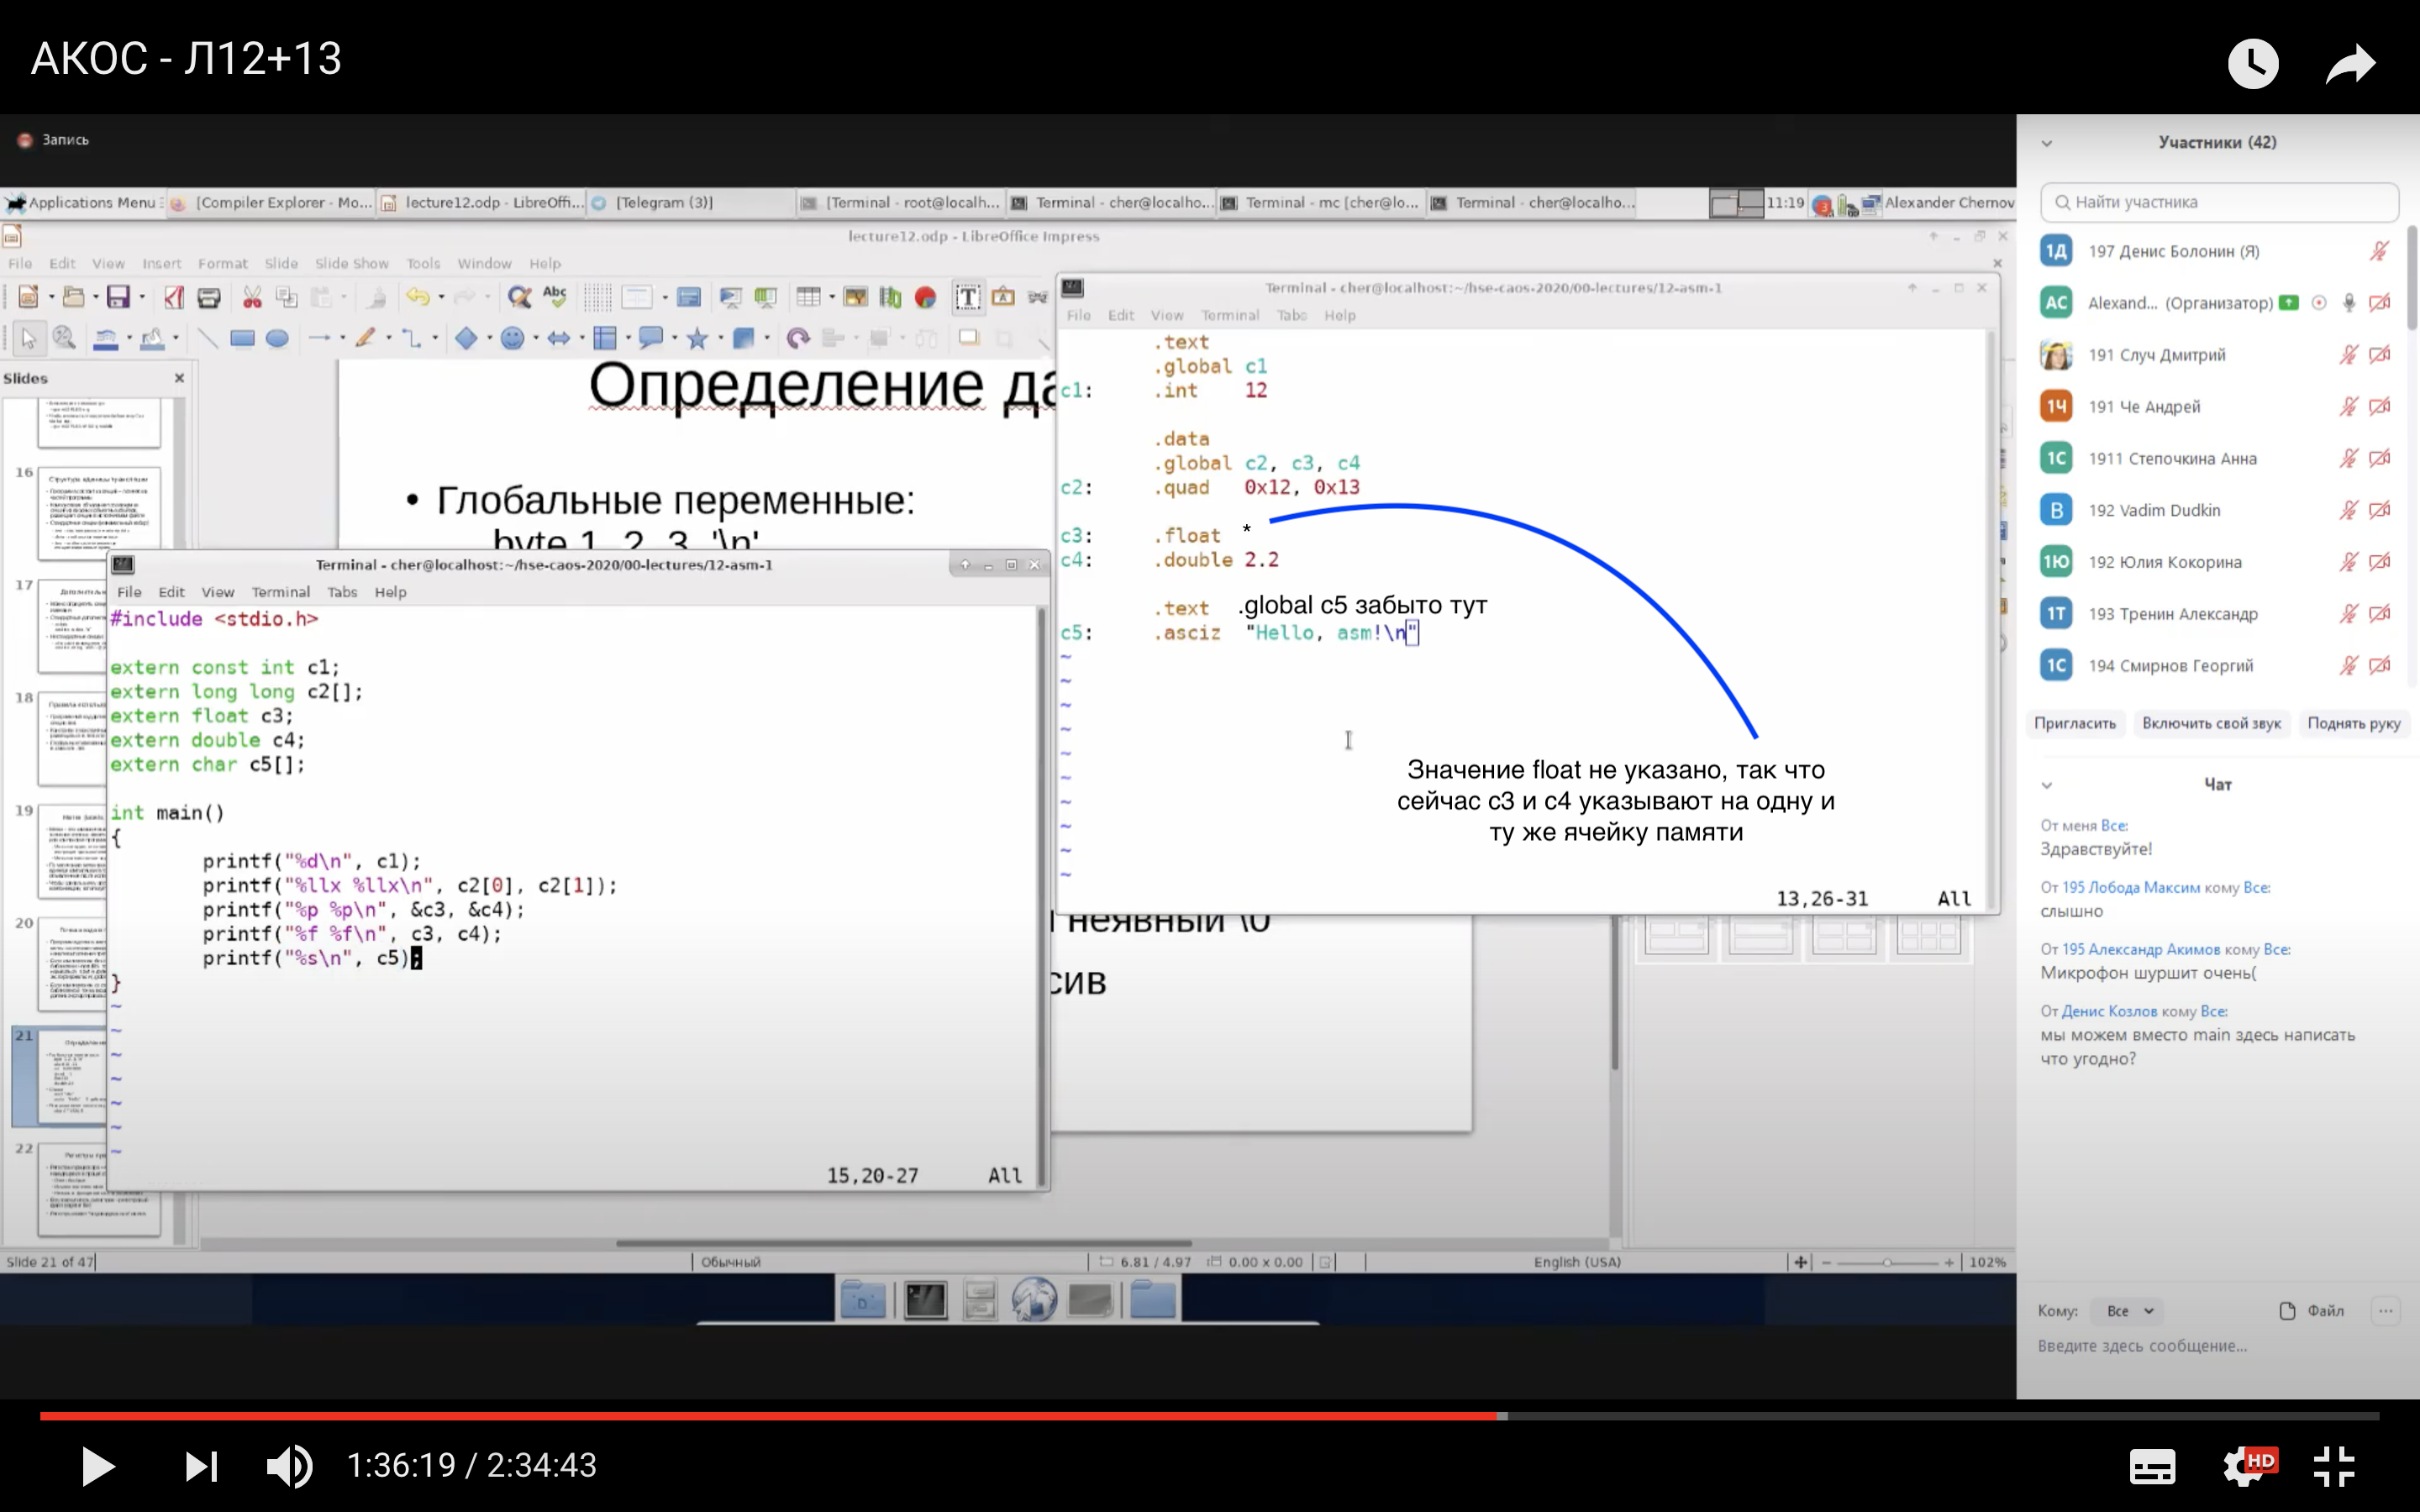
\includegraphics[scale=0.3]{./pic03.png} \\
    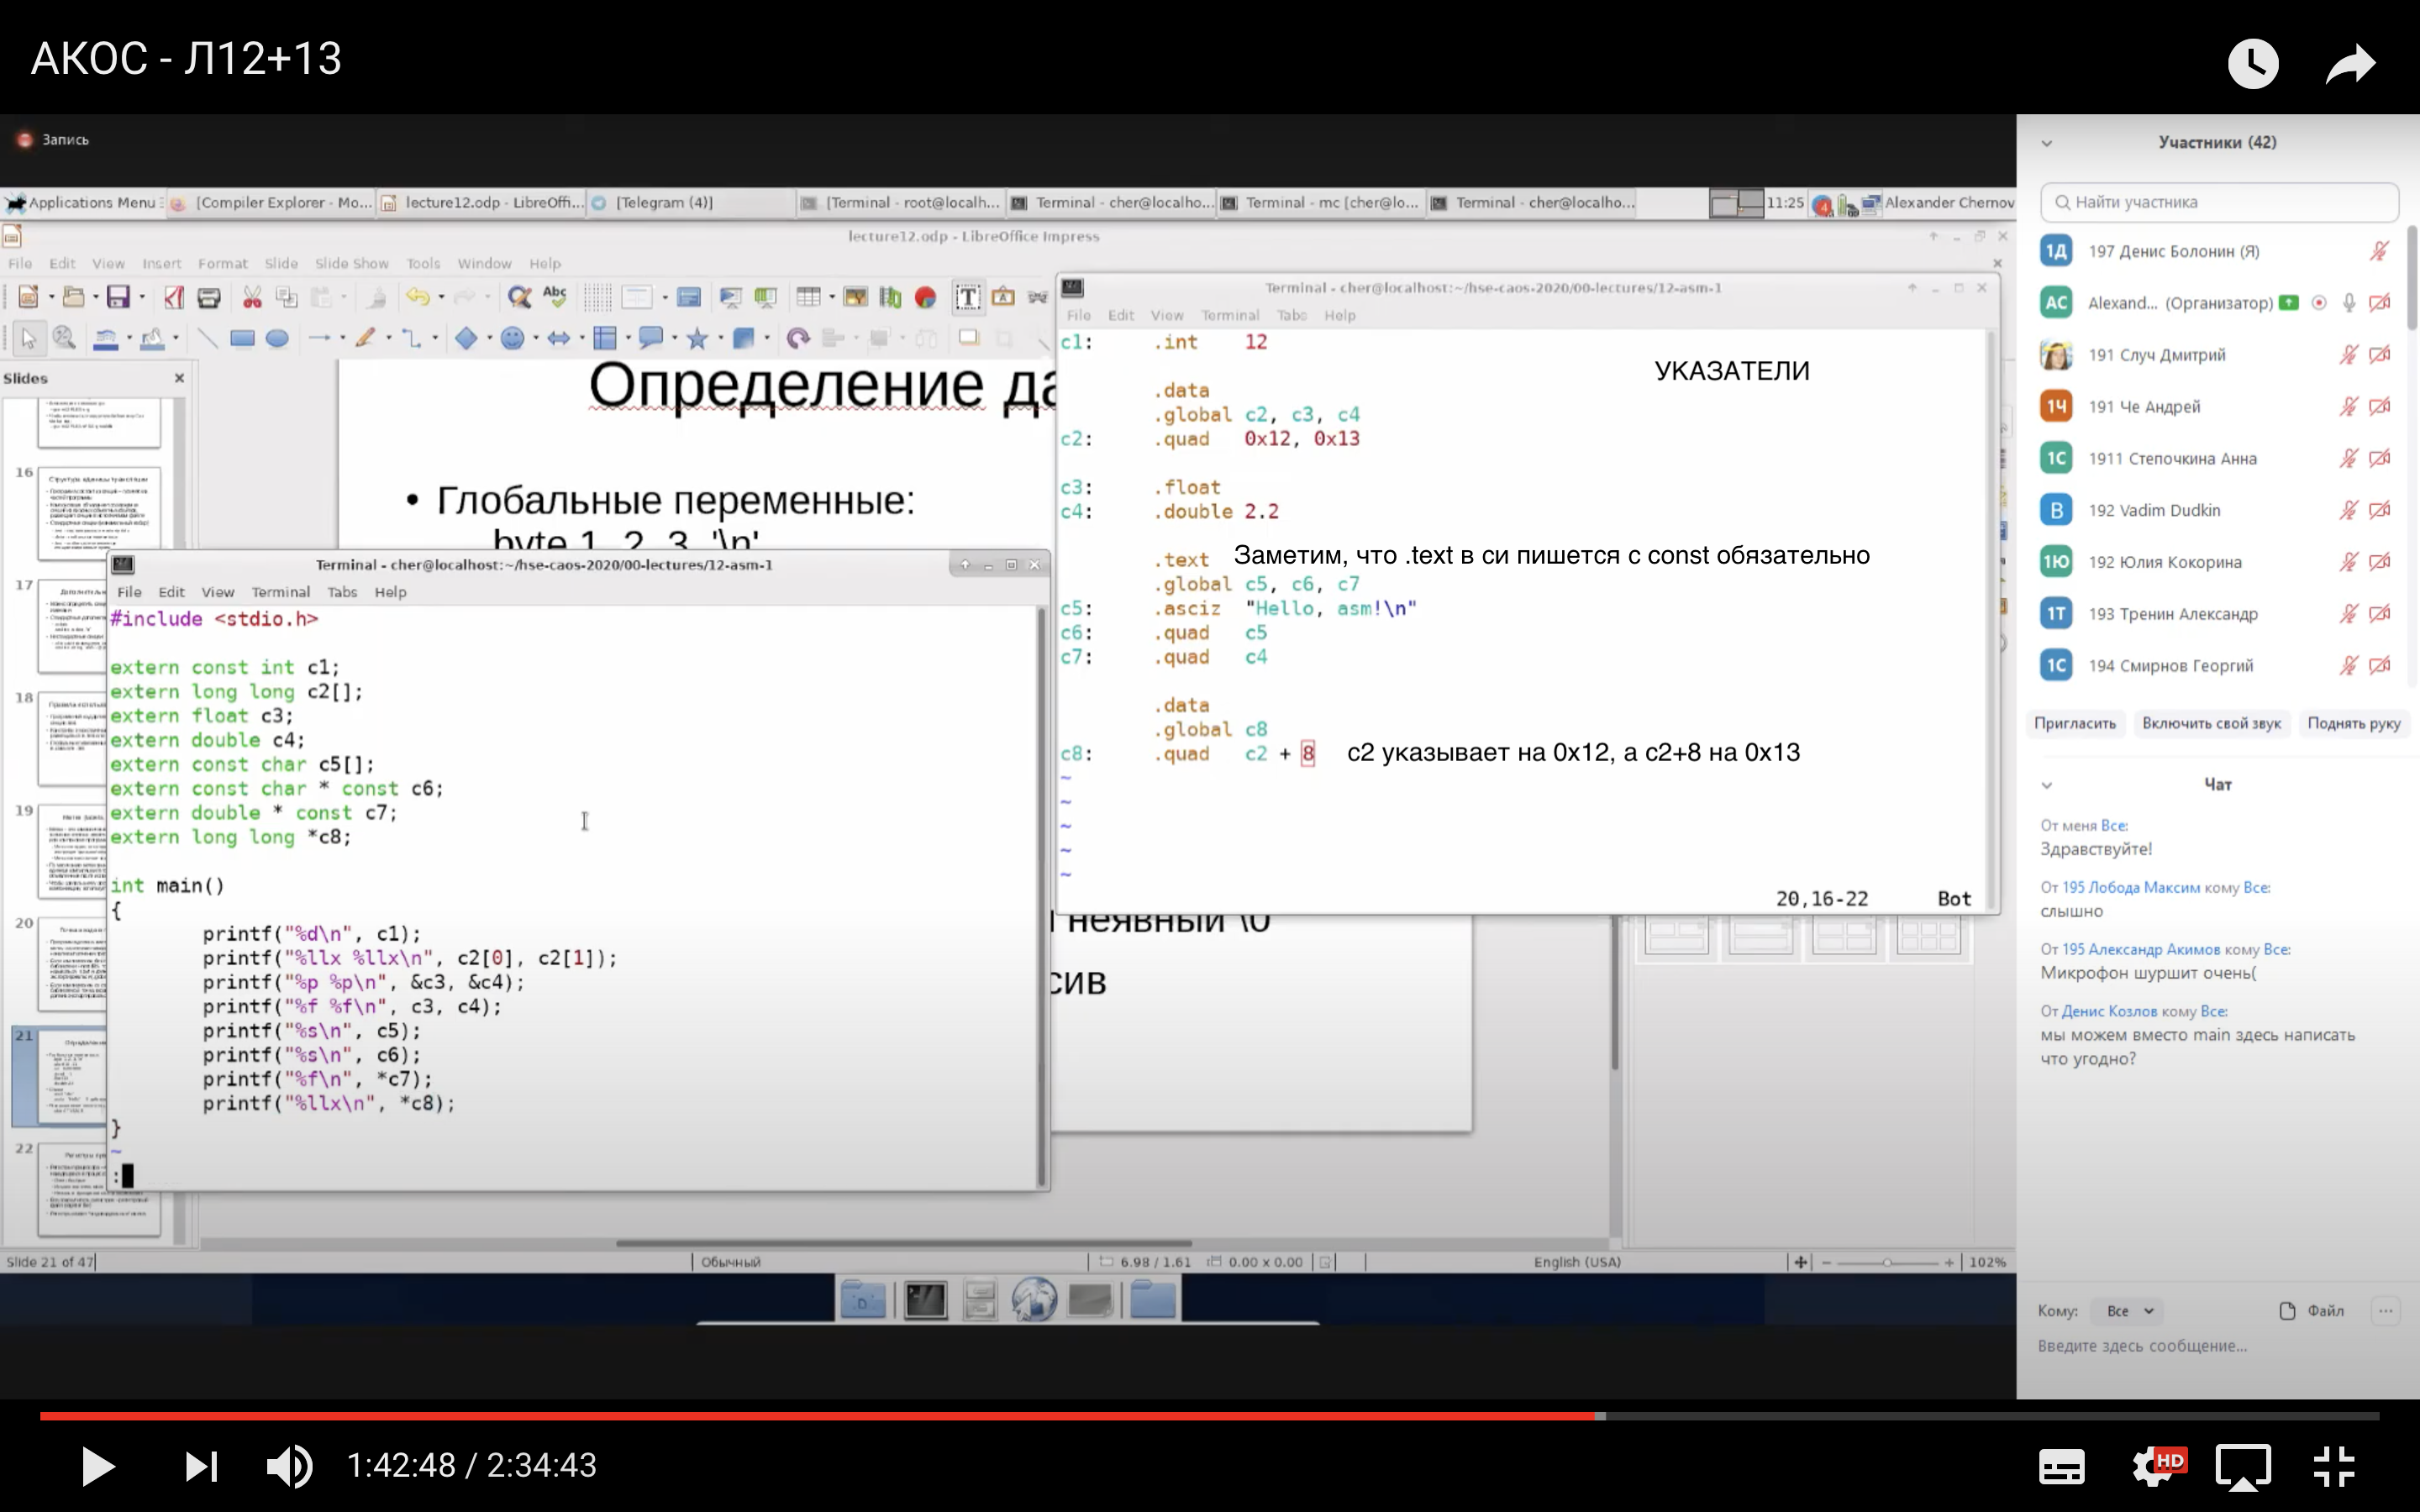
\includegraphics[scale=0.3]{./pic04.png} \\

\subsection{Регистры}
\textbf{Регистры} - ячейки памяти, находящиеся в процессоре, непосредственно там, где происходят вычисления. \\
Как правило, регистров мало или очень мало. И процессоры умеют выполнять операции только над значениями, которые записаны в регистрах. \\
Важная особенность регистров - они глобальные, то есть одни и те же на всех подпрограммах. 
\\
\\
Для более эффективного размещения функций, для их более эффективного выравнивания рекомендуется выравнивать код по границе 16 байт, то есть написать ".align 16" - не понял, НО ЗАПИСАЛ СЛОВО В СЛОВО 


\end{document}